

\begin{figure}[t]
\centering
  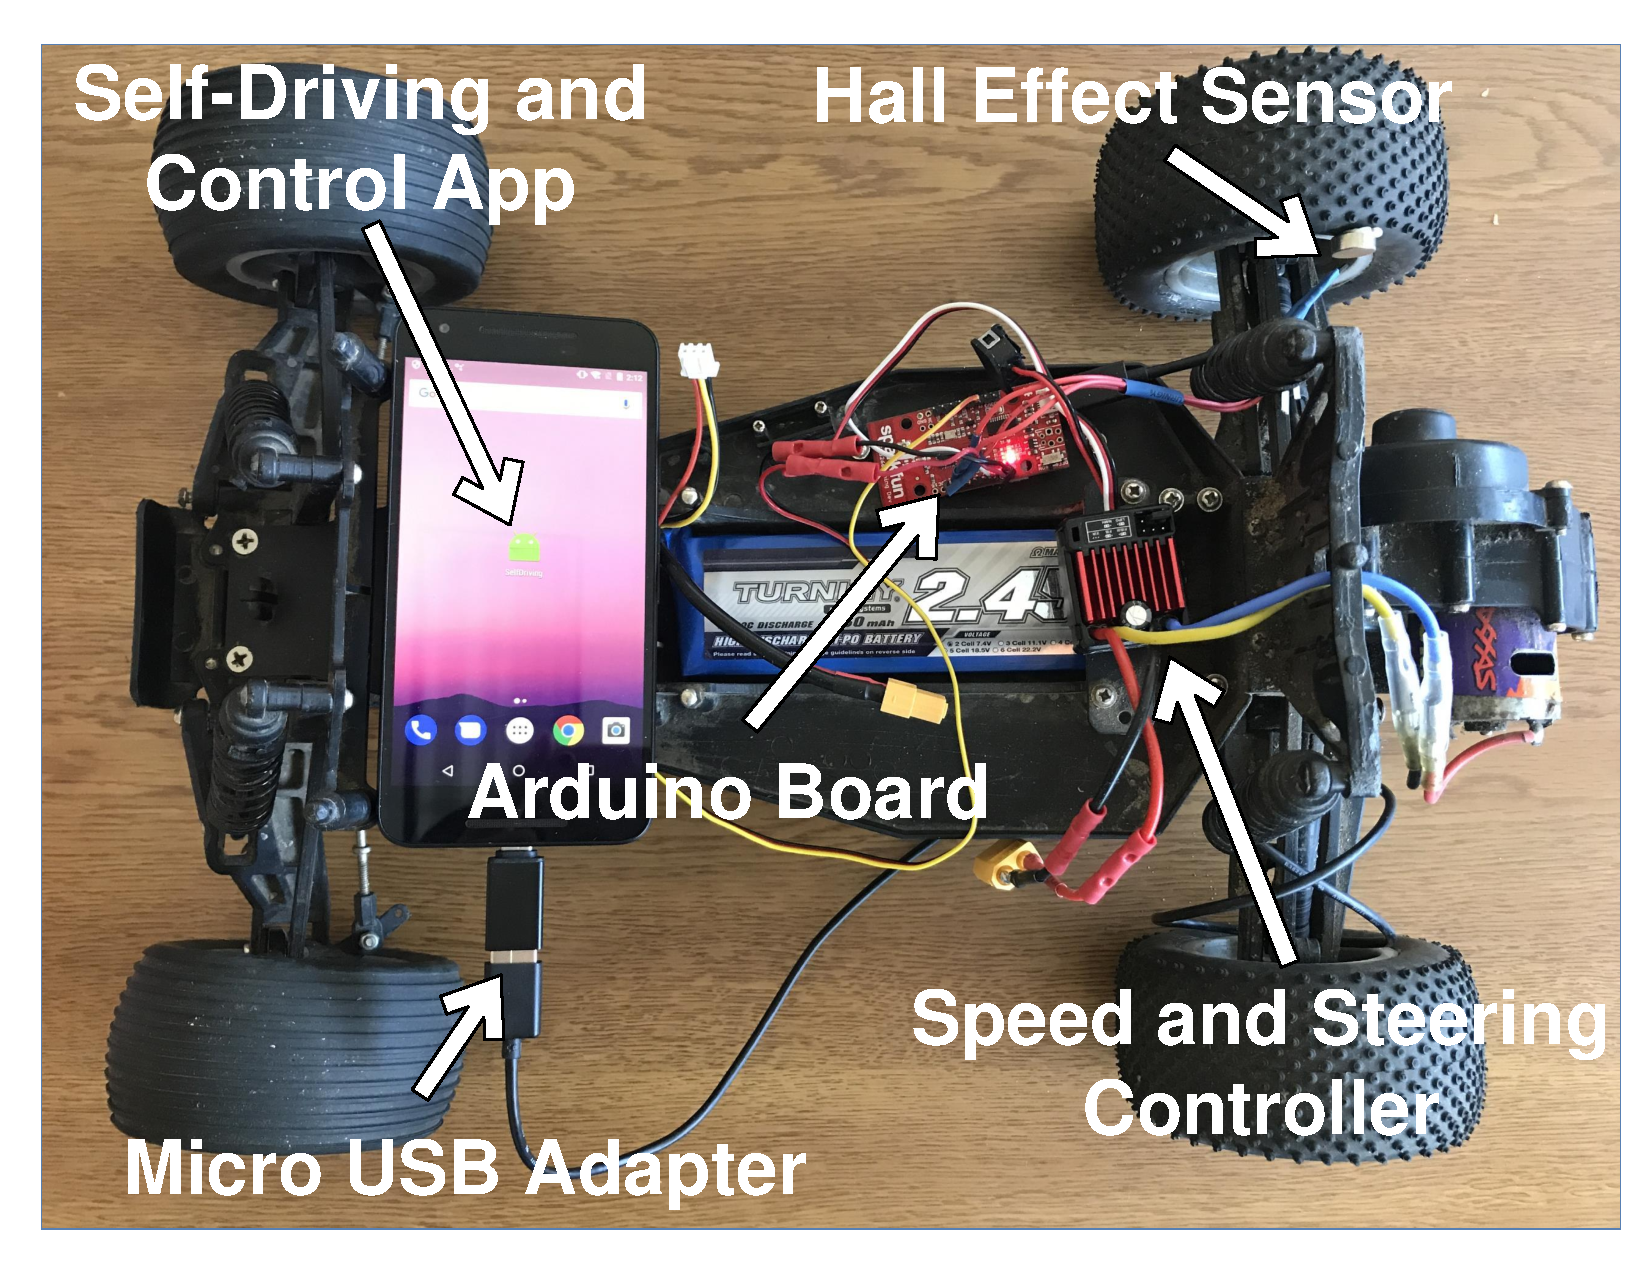
\includegraphics[width=4.0in,angle=0]{Figs/RTDrive/rc_car.pdf}
\vspace{-0.2cm}
\caption{The vehicle testbed.}
\vspace{-0.5cm}
\label{rc_vehicle}
\end{figure}

\begin{figure}[!ht]
\centering
  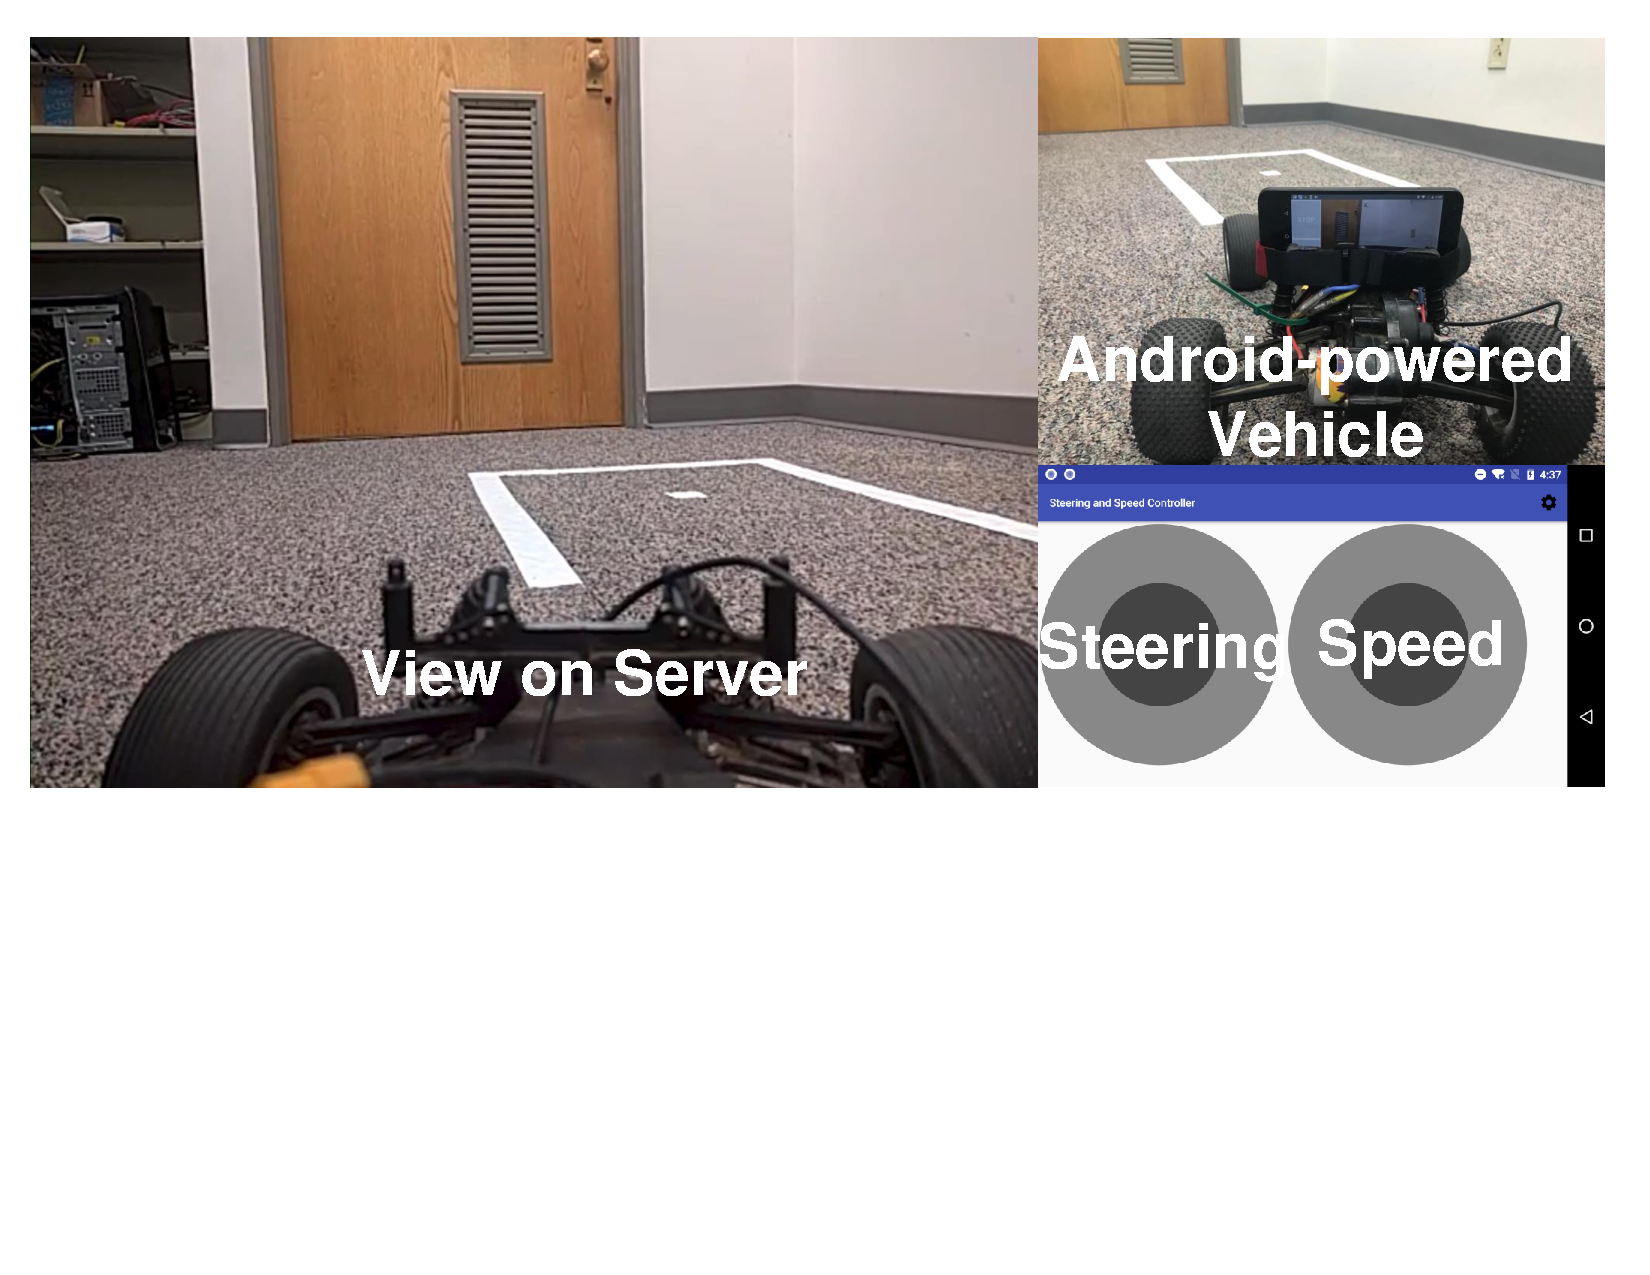
\includegraphics[width=4.0in,angle=0]{Figs/RTDrive/rc_car_cropped.pdf}
\vspace{-0.2cm}
\caption{The live streaming and remote control platform.}
\vspace{-0.2cm}
\label{platform}
\end{figure}


The framework consists of two parts, an Android-powered 
self-driving vehicle and a remote control server. 
The customized remote control vehicle
and the overview of the entire platform are illustrated in Fig. \ref{rc_vehicle} and Fig. \ref{platform}.


The self-driving and streaming client is implemented as
Android application. 
The self-driving and control app compress the video by using 
video compression standard H.264 or MPEG-4 \cite{marpe2006h}.  
Meanwhile, it identifies lane markers by using OpenCV
library and customized detection algorithms. 
The lane markers detection modules are implemented
in C/C++ and the interfaces are exported to upper 
layer through Java Native Interface (JNI).  
In the Android-powered self-driving system, 
the app transfers the control message to the
Arduino board through a Micro USB cable. 
A Hall Effect Sensor is installed to track vehicular speed
by recording the number of wheel rotations per second. 
The Arduino board bridges the Android app and the hardwares, 
i.e., the steering controller and hall effect sensor. 


The multi-thread and event-driven remote control 
server is implemented in C++.  
One UDP thread to used to receive the video stream from the
self-driving vehicle. 
The UDP thread sends the compressed video data to a GStreamer
pipeline \cite{gstreamer} running in another thread. 
The GStreamer pipeline decompresses, displays and records the video.   
There is another thread receives control message from a customized
controller to control the vehicle by human operator.


There are totally 2700+ lines of Java code for Android app implementation
and 3200+ lines of C/C++ code for the remote server.
The minimum Android SDK version is 21, which is the minimum requirement
of OpenCV3.2 SDK for Android platform. 
The Android phone we use is Nexus 5x. 
It has a reversed camera sensor and we have to rotate the camera by 180 degree
programmatically. 
The remote server is implemented on Ubuntu 16.04. 
The GStreamer version we use is 1.0. 

